\section{Patrones de diseño}


\begin{itemize}
\item Se nombran solo algunos patrones de diseño, hay un montón. Estos se descubren con el tiempo. Una lista con muchos patrones \href{https://java-design-patterns.com/patterns/}{aquí}.
\item Es buena practica usar nombres que relacionen a los patrones usados.
\end{itemize}

\medskip
\textit{Libro muy recomendado: Design Patterns - Erich Gamma}

\subsection*{Patrones creacionales}
\begin{itemize}
\item Las abstractas arriba, las dependientes - inestables - abajo. Esto muestra la inversión en la cadena de dependencia.
\item Se usan cuando hay que aislar la creación de instancias.
\item Resuelven el encapsulamiento, ocultan y ordenan la creación de instancias, vuelven al sistema independiente del proceso de creación.
\item No publicar cuestiones que no le interesa a otro paquete.
\item Se vuelven mas importantes a medida que se pasa de usar herencia a composición de objetos.
\item Nos dan mucha flexibilidad en cuanto a que se crea, quien lo crea, como es creado, y cuando se crea.
\end{itemize}


\subsubsection*{Factory Method}
\begin{itemize}
\item La forma más simple de ocultar la creación de un objeto es usando un método que devuelve un objeto.
\item Si aparecen nuevas clases del tipo1, extendemos la de la fabrica original, de manera tal de ocultar la creación de cada uno de los tipos en métodos de las clases diferentes.
\item Presenta la dificultad de mantener 2 jerarquías de clases en paralelo.
\item Se bautiza como factory method a cualquier clase que tenga un método para crear otro objeto y devolverlo.
\item Su intención es crear una interfaz para la creación de un objeto que permita a las subclases decidir que clase instanciar.
\item Elimina la necesidad de atar clases especificas de la aplicación al código.
\item Crear en una manera descriptiva las instancias los que no son descriptivos. (\textit{Clase con muchos constructores, se complica elegir cual. Necesitamos sacar la ambigüedad de esto. Una forma de arreglar esto es proveer métodos de clase que tengan nombres descriptivos y constructores protegidos. Cada uno de los métodos seria un factory method. (no es la version propuesta por Gamma, es valida igual. )}) - \href{https://github.com/brunograssano/Algoritmos_3_TP2_PM2/blob/master/src/main/java/edu/fiuba/algo3/modelo/preguntas/FabricaDePreguntas.java}{Ejemplo}
\end{itemize}

\begin{figure}[!htb]
    \centering
    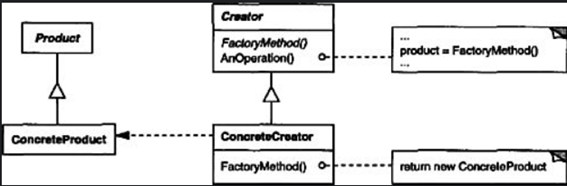
\includegraphics[width=0.8\textwidth]{img/FactoryMethod.png}
\end{figure}

\subsubsection*{Abstract Factory}
\begin{itemize}
\item Logramos un esquema en el cual se crean objetos concretos sin violar la inversión de la dependencia.
\item Busca proveer una interfaz para crear familias de objetos relacionados o dependientes entre si sin especificar la clase en concreto.
\item Se usa cuando un sistema debe de ser independiente de como se crean los objetos, cuando un sistema debe de configurarse con una familia de objetos de muchas.
\item Aísla las clases concretas. Los clientes interactúan solo con la interfaz.
\item Vuelve fácil el cambio de productos de familias.
\item Promueve consistencia entre los productos.
\item Se vuelve difícil soportar nuevos tipos de productos. Esto es porque la interfaz de la abstract factory fija el conjunto de productos.
\end{itemize}

\begin{figure}[!htb]
    \centering
    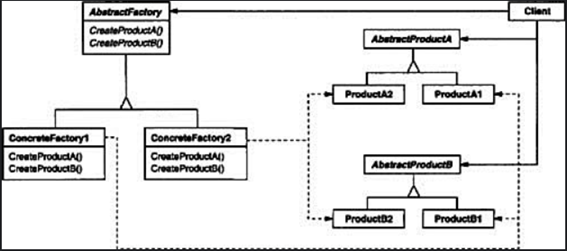
\includegraphics[width=0.8\textwidth]{img/AbstractFactory.png}
\end{figure}

\subsubsection*{Prototype}
\begin{itemize}
\item En vez de crear clona objetos. Nos evita tener que mantener la jerarquía paralela de la factory. (Variante del Abstract Factory)
\item La intención es especificar los tipos de objetos a crear a partir de un prototipo, y crear nuevos objetos a partir de copiar el prototipo.
\item Se usa cuando un sistema debe de ser independiente de como sus productos son creados, las clases de productos a instanciar se especifican en tiempo de ejecución, se quiere evitar jerarquías de fabricas paralelas a la de productos,  las instancias de una clase solo pueden tener pocas combinaciones de estado..
\item Esto esconde las clases concretas del cliente.
\item Se pueden agregar y quitar prototipos en tiempo de ejecución.
\item Reduce las subclases
\end{itemize}

\begin{figure}[!htb]
    \centering
    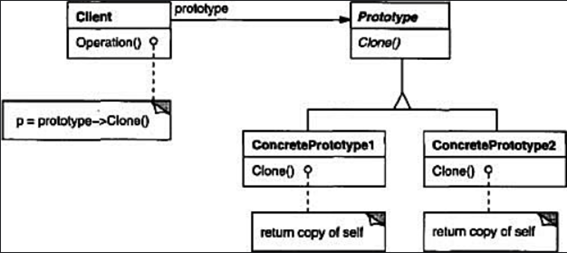
\includegraphics[width=0.8\textwidth]{img/Prototype.png}
\end{figure}

\subsubsection*{Builder}
\begin{itemize}
\item Variante del abstract factory. Cuando invoco a crear un objeto, invoca a la creación de cada parte del objeto complejo.
\item Busca separar la construcción de un objeto complejo de la representación, de forma tal de que el mismo proceso cree diferentes representaciones.
\item Se usa cuando el algoritmo de creación deba de ser independiente del objeto y la construcción deba de permitir diferentes representaciones.
\item Esto permite cambiar la representación interna de un producto y esconde la representación interna del producto con la interfaz.
\item Aísla el código para construcción y representación. Esto mejora la modularidad al encapsular el proceso.
\item Nos da un control mas fino sobre el proceso de creación. (Lo hace al objeto paso a paso)
\end{itemize}

\begin{figure}[!htb]
    \centering
    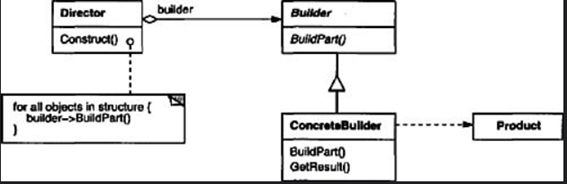
\includegraphics[width=0.8\textwidth]{img/Builder.png}
\end{figure}

\begin{figure}[!htb]
    \centering
    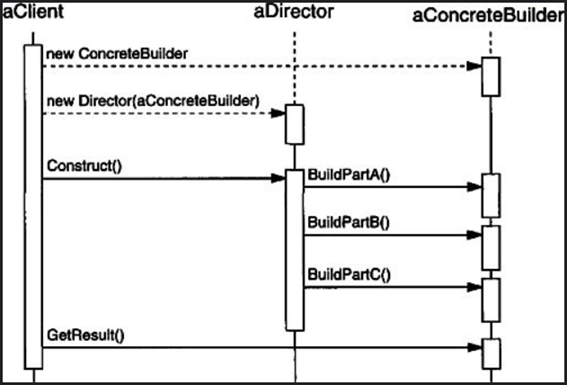
\includegraphics[width=0.8\textwidth]{img/Builder2.png}
\end{figure}

\subsubsection*{Singleton}
\begin{itemize}
\item Se usa cuando se quiere que exista una única instancia de una clase y proveer un único punto de acceso a ella.
\item Permite un punto de accesos controlado.
\item Es una mejora respecto de variables globales. (En cierta forma lo es todavía)
\item Permite variar el numero de instancias.
\item Es mas flexible que métodos de clase.
\item Se puede extender la clase.
\item Los usos mas frecuentes son en caches, configuraciones y pulls.
\end{itemize}

\begin{figure}[!htb]
    \centering
    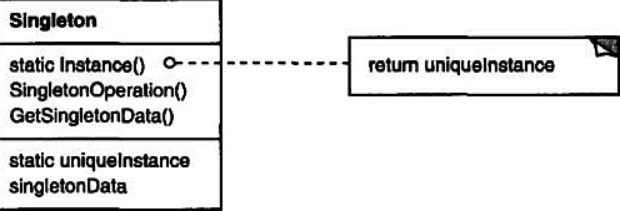
\includegraphics[width=0.8\textwidth]{img/Singleton.jpg}
\end{figure}


\subsection*{Patrones de organización del trabajo - Behavioral Patterns}
\begin{itemize}
\item Estos patrones conviene usarlos cuando hay que repartir las responsabilidades entre objetos.
\end{itemize}


\subsubsection*{Command}
\begin{itemize}
\item La intención es encapsular la acción de un objeto.
\item Se usa cuando se quiere parametrizar objetos mediante una acción a ejecutar, especificar, encolar, y ejecutar acciones en diferentes momentos, soportar deshacer la operación.
\item Desacopla el objeto que solicita un servicio de aquel que lo presta. Versión en objetos de una función Callback
\item Se pueden componer comandos con un composite.
\item Se vuelve fácil agregar nuevos comandos, no se tiene que cambiar clases existentes.
\end{itemize}


\begin{figure}[!htb]
    \centering
    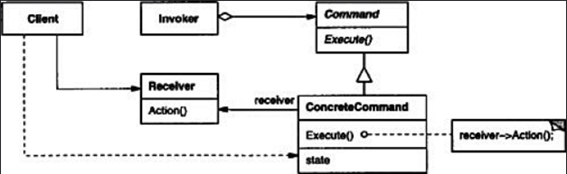
\includegraphics[width=0.8\textwidth]{img/Command.png}
\end{figure}

\subsubsection*{Chain of Responsability}
\begin{itemize}
\item La intención es desacoplar quien envía un mensaje de quien lo ejecuta. Los objetos lo van pasando.
\item Se usa cuando mas de un objeto puede manejar un mensaje y este objeto no se conoce a priori, se quiere mandar un mensaje a varios objetos sin especificar cuales en especifico, el conjunto de objetos que manejan el mensaje se especifica dinámicamente.
\item Va pasando la posta hasta que lo trate alguien. Desacoplar quien solicita un servicio de un conjunto.
\item Se puede ver también como una función de orden superior que toma una función, y si no puede resolver lo delega a la función.
\item Reduce el acoplamiento. Libera a los objetos del saber quien lo va a manejar al mensaje.
\item Da flexibilidad en asignar responsabilidades a los objetos.
\item El receptor no esta garantizado, por lo que puede no ejecutarse si no se configura correctamente.
\end{itemize}

\begin{figure}[!htb]
    \centering
    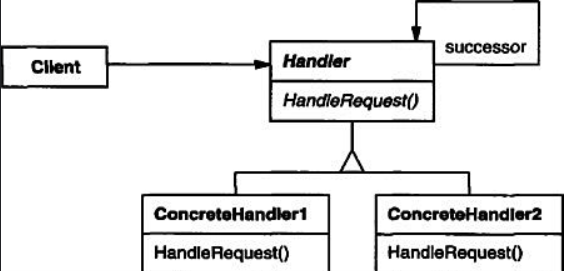
\includegraphics[width=0.8\textwidth]{img/ChainOfResponsability.png}
\end{figure}

\subsubsection*{Mediator}
\begin{itemize}
\item La intención es definir un objeto que encapsule como un conjunto de objetos interactúan.
\item Se usa cuando un conjunto de objetos se comunican de forma bien definida pero compleja.
\item Busca evitar una cantidad de dependencias enormes entre todos los componentes. Este mediador elimina las dependencias cruzadas, pero tiene la desventaja de que todos conocen al mediador, y que el mediador conoce a todos (Tenemos una dependencia circular). Es fácil agregar componentes adicionales porque la lógica esta concentrada en el mediador.
\item Limita las subclases. Localiza todo el comportamiento que estaría distribuido.
\item Desacopla los collegues.
\item Vuelve mas abstracto como cooperan los objetos.
\item Centraliza el control.
\item No es necesario definir la clase abstracta mediator en la implementación.
\end{itemize}

\begin{figure}[!htb]
    \centering
    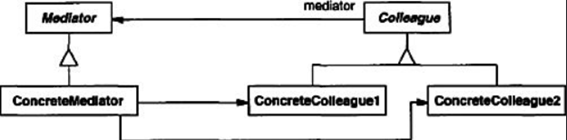
\includegraphics[width=0.8\textwidth]{img/Mediator.png}
\end{figure}

\begin{figure}[!htb]
    \centering
    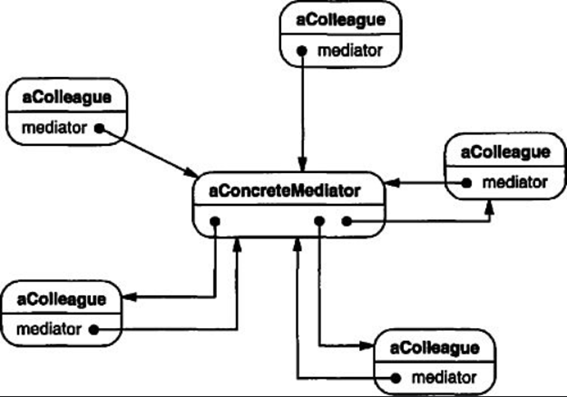
\includegraphics[width=0.6\textwidth]{img/Mediator2.png}
\end{figure}

\subsection*{Patrones de control de acceso}

\begin{itemize}
    \item Se encargan sobre como las clases y objetos se componen para formar estructuras mas grandes. (Structural Patterns)
    \item Compone objetos para lograr nuevas funcionalidades. (Structural Patterns)
\end{itemize}

\subsubsection*{Facade (Structural Patterns)}
\begin{itemize}
\item La intención es proveer una interfaz unificada a un conjunto de interfaces de un subsistema.
\item Se usa cuando queremos una interfaz simple a un subsistema complejo, hay muchas dependencias entre clientes y la implementación de las clases de una abstracción, queremos una capa entre los subsistemas (entry point).
\item Escribimos código para acceder servicios externos y no contaminar el contexto de nuestro sistema. Aparece la segregación de interfaces.
\item Tener un acceso de mas alto nivel.
\item Reducir el acoplamiento.
\item Protege a los clientes de las componentes de los subsistemas.
\item Promueve weak coupling entre los subsistema y los clientes.
\item No previene a las aplicaciones el uso de los subsistemas si quieren. Permite elegir entre la facilidad de uso y la generalidad.
\end{itemize}

\begin{figure}[!htb]
    \centering
    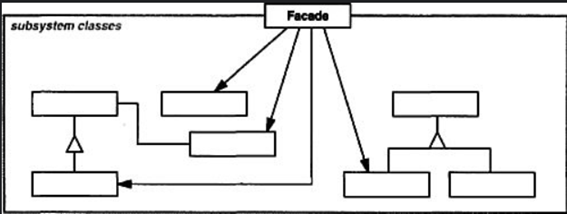
\includegraphics[width=0.8\textwidth]{img/Facade.png}
\end{figure}

\begin{figure}[!htb]
    \centering
    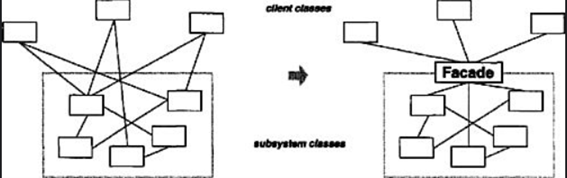
\includegraphics[width=0.8\textwidth]{img/Facade2.png}
\end{figure}

\subsubsection*{Proxy (Structural Patterns)}
\begin{itemize}
\item Su intención es proveer un sustituto a otro objeto para controlar el acceso.
\item En los métodos de proxy se decide que puede hacer la clase que llama respecto de la clase oculta.
\item Controla acceso a determinados tipos de recursos, esto posterga el costo de la creación e inicialización hasta que se necesite.
\item Proxy remoto para objetos separados de lugar.
\item Proxy virtual: Se usa en las arquitecturas de tipo EA. Lazy load, creo en memoria un proxy, el cliente se cree que tiene un objeto completo, pero en realidad voy trayendo lo que necesito a medida que se pide.
\item El proxy dio lugar al garbage collector, de alguna manera controla la creación y destrucción de objetos.
\end{itemize}

\begin{figure}[!htb]
    \centering
    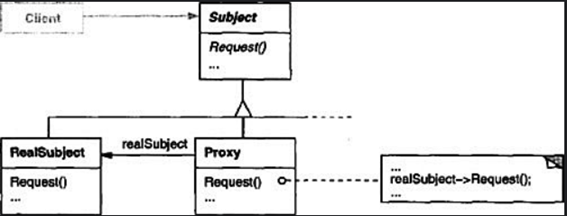
\includegraphics[width=0.8\textwidth]{img/Proxy.png}
\end{figure}

\subsubsection*{Iterator (Behavioral Patterns)}
\begin{itemize}
\item La motivación es proveer una forma de acceder a los elementos de un aggregate object se forma secuencial sin exponer la representación.
\item Permite múltiples formas de recorrer el objeto.
\item Provee una interfaz uniforme para el recorrido. (polymorphic iteration)
\item Sirve para no exponer los datos de una colección directamente, los accedo a través de un iterador.
\end{itemize}

\begin{figure}[!htb]
    \centering
    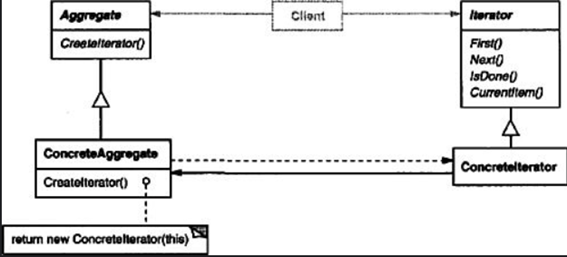
\includegraphics[width=0.8\textwidth]{img/Iterator.png}
\end{figure}


\subsection*{Variación de servicio}
Quiero resolver que objetos de determinadas clases tengan un comportamiento distinto.


\subsubsection*{Strategy (Behavioral Patterns)} 
\begin{itemize}
\item Se usa cuando tengo muchas formas de hacer una cosa. Se dice que encapsula un algoritmo y permite variarlo independientemente de los clientes..
\item Cambia el algoritmo completo.
\item Recibe el contexto que es la clase que se va a usar. Contiene la información necesaria para resolver la estrategia.
\item Se aprovecha en tiempo de ejecución.
\item De acuerdo a la estrategia que use estoy variando lo que hago.
\end{itemize}


\begin{figure}[!htb]
    \centering
    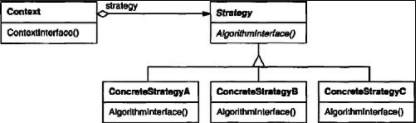
\includegraphics[width=0.8\textwidth]{img/Strategy.PNG}
\end{figure}


\subsubsection*{Template Method}
\begin{itemize}
\item El algoritmo esta prefijado, el esqueleto de este.
\item Cada una de las clases redefinen el paso correspondiente.
\item El objeto instanciado ejecuta el algoritmo.
\item Muy usado en los frameworks.
\item Se trata de tener diversidad y resolverlo en tiempo de compilación.
\item Variación de servicio en tener la posibilidad al instanciar un objeto de variar los pasos.
\item Fundamental para reusar código.
\end{itemize}


\begin{figure}[!htb]
    \centering
    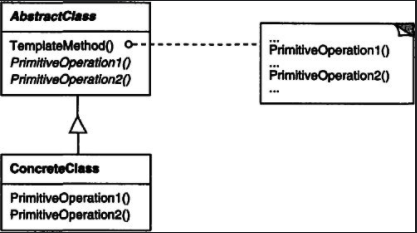
\includegraphics[width=0.5\textwidth]{img/TemplateMethod.PNG}
\end{figure}

\subsubsection*{State (Behavioral Patterns)}
\begin{itemize}
\item Tiene que ver con que los objetos se comporten de acuerdo al estado en que están.
\item El estado de un objeto depende de su historia. Desde que lo inicializamos.
\item Un indicativo de usar el patrón es cuando aparecen muchas condiciones.
\item Maquina de estados para realizar los cambios sin que se conozcan entre si los estados. Usa una lookup table que conoce a todos los estados concretos.
\item Puede tener un contexto que le pase lo que necesita al estado, o incluso pasarse a si mismo.
\item Como resultado del patrón, se ubica el comportamiento especifico en diferentes particiones para cada estado. (Puede llegar a introducir muchas clases, sin el patrón se tendrían condicionales)
\end{itemize}


\begin{figure}[!htb]
    \centering
    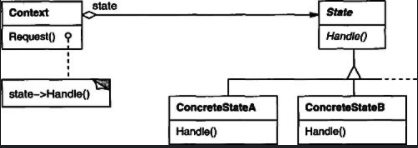
\includegraphics[width=0.8\textwidth]{img/State.PNG}
\end{figure}

\subsection*{Extensión de servicio}
Quiero que los objetos de mi clase hagan lo que hacían y algo mas.

\subsubsection*{Decorator}
\begin{itemize}
\item Esta orientado a objetos 'livianos'. Que encapsulen comportamiento más que atributos.
\item El decorador extiende el servicio en tiempo de ejecución, le agrega o quita responsabilidades. (dinámico)
\item Decorador puede tener clases hijas que redefinan su comportamiento.
\item Es mucho más flexible que la herencia.
\item Podemos decorar múltiples veces el mismo objeto. (a objetos individuales, no a clases enteras)
\item Da mucha reusabilidad.
\item Generalmente se usa con Composite.
\item Un sistema que usa Decorator generalmente termina lleno de un montón de objetos pequeños que se parecen entre si.
\end{itemize}


\begin{figure}[!htb]
    \centering
    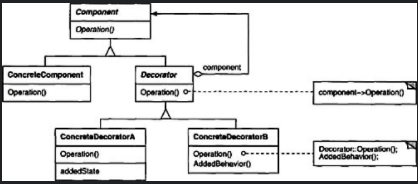
\includegraphics[width=0.8\textwidth]{img/Decorator.PNG}
\end{figure}

\subsubsection*{Visitor}
\begin{itemize}
\item Lo usamos para agregar métodos/funciones a una clase.
\item Se dice que es un double dispatch.
\item Representa una operación que se ejecuta en los elementos de una estructura. Permite crear esta operación sin tener que cambiar las clases de los elementos. en los que opera.
\item Se puede usar cuando un objeto contiene muchas clase de objetos con diferentes interfaces y queremos realizar acciones que dependen de las clases concretas.
\end{itemize}


\begin{figure}[!htb]
    \centering
    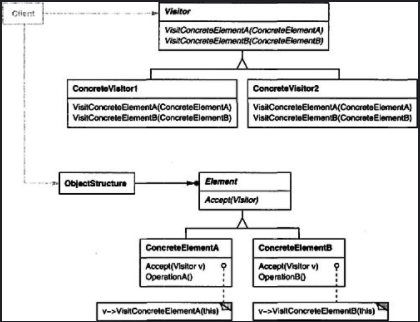
\includegraphics[width=0.8\textwidth]{img/Visitor.PNG}
\end{figure}

\subsection*{Varios}

\subsubsection*{Bridge}
Cuando se deba desacoplar abstracciones de implementaciones
Los métodos de las abstracciones delegan en las implementaciones
Se complementa con algún patrón creacional.
Cambios en la implementación de una abstracción no debería de impactar a los clientes.
Oculta detalles a los clientes.
Se puede extender fácilmente.

\begin{figure}[!htb]
    \centering
    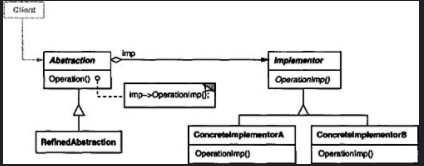
\includegraphics[width=0.8\textwidth]{img/Bridge.PNG}
\end{figure}

\subsubsection*{Adapter}
\begin{itemize}
\item Esta orientado a reutilizar código.
\item Cuando es necesario adaptar una clase para que funcione en el contexto que necesito.
\item Suele usarse para adaptar los métodos de algún sistema externo que estamos usando para que un facade acceda a ese sistema.
\item Convierte una interfaz en otra que espera el cliente.
\item Se pueden usar Adapters de dos direcciones para agregar transparencia (generalmente no son transparentes a todos los clientes)
\end{itemize}


\begin{figure}[!htb]
    \centering
    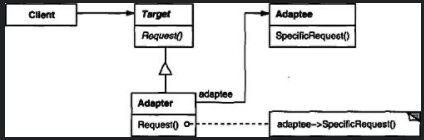
\includegraphics[width=0.8\textwidth]{img/Adapter.PNG}
\end{figure}

\subsubsection*{Composite}
\begin{itemize}
\item Esta orientado a ofrecerle al cliente una misma interfaz para que un objeto se trate de un único objeto o una colección de objetos.
\item Ejemplos de uso se ven en procesamiento de texto y filtros.
\item Compone objetos en estructuras - similares a arboles - para representar jerarquías.
\item Como se vuelve indistinguible al grupo de objetos de un solo objeto, simplifica al cliente. Esto trae una desventaja también, si el diseño se vuelve muy general se complica agregar restricciones a los componentes del composite.
\item Para maximizar esta indistinguibilidad, se debe de agregar la mayor cantidad posible de métodos comunes en la interfaz. (Puede llevar a entrar en conflicto con la separación de lo que corresponde a cada clase)
\end{itemize}


\begin{figure}[!htb]
    \centering
    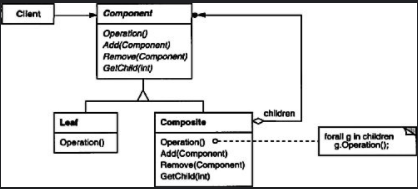
\includegraphics[width=0.8\textwidth]{img/Composite.PNG}
\end{figure}